\chapter{Background}
\label{background}
This chapter gives a concise introduction into the basic topics of this work. First, the main aspects of parallel programming are explained, in order to give the reader the essential knowledge that is mandatory to understand the problem tackled by this thesis. After that, the embedded domain and the tools that are used to create software for it (\textit{mbeddr} and \textit{C}) are presented.

\section{Parallel Programming}
Parallel programming is a technique to speed up the classical sequential execution of programs which are suited for parallelization in the limits of \textit{Amdahl's law} \cite{Amdahl}\cite{MathematicalLimits}. The law gives an upper bound on the possible speed up of an algorithm based on the amount of parallelizeable code.\footnote{This work, however, is not about finding appropriate patterns for this purpose but about giving a generic approach. Thus, \textit{Amdahl's law} will not be further considered.} The pitfalls of the often mandatory communication in parallel programming arise from race conditions and countermeasures thereof.

\subsubsection{Processes and Threads}
Every program in execution which may be delayed or interrupted is represented by a process. A process typically has its own protected data (via virtual memory) and execution state and consists of one or more threads. A thread, also known as lightweight process, shares some of the memory with its process but has its own execution state and thread-local storage as needed \cite[p.~20]{PrinciplesOfModernOSs}. In the course of programming language and operating system development, several variants of threads have been devised, among others green threads, fibers and coroutines which mainly differ in how they are managed.

\subsubsection{Parallelism and Concurrency}
If multiple threads are ``in the middle of executing code at the same time'' \cite[p.~14]{MultiProgWithJavaTech} they are processed concurrently. They can be executed at the same time on different processors or interleaved on a single processor, which means that they are executed in an alternating way. The former is also called parallelism. Parallelism, generalized to ``the quality of occurring at the same time'' \cite[p.~91]{OSs_AConceptBasedApproach}, can manifest in at least four different ways: From an application programmer's view there exist bit-level parallelism and instruction-level parallelism at a very low level. Bit-level parallelism is concerned with increasing the word size of processors in order to reduce the amount of cycles that are needed to perform an instruction \cite[p.~15]{ParCompArchitecture_HW/SW_Approach}. Instruction-level parallelism, also called pipelining, is the simultaneous utilization of multiple stages of the processor's execution pipeline. Both bit-level parallelism and instruction-level parallelism primarily reside on the hardware level and the operating system level and thus are irrelevant to this work. Data parallelism is present if the same calculation is performed on multiple sets of data. It can be regarded as a specialization of task parallelism, which denotes the simultaneous execution of different calculations ``on either the same or different data'' \cite[p.~125]{ParCompArchitecture_HW/SW_Approach}. This work focuses on the latter form of parallelism, since it is the more general approach to application-level parallelism.

\subsubsection{Implicit vs. Explicit Parallelism}
Another way to distinguish parallelism is the way it is expressed in the programmer's code. Traditionally, the programmer has to define explicitly how and when parallelization shall be performed and where communication between separate units of execution takes place. Instead, with implicit programming, the programmer declares dependencies between data and the compiler uses this information to detect parallelizable code segments which it may then be executed in parallel \cite[p.~334]{ParallelScientificComputing}.

\subsubsection{Data Races}
When a process consists of multiple concurrently running threads which have access to the shared data of their process, a class of errors that is unique to parallel (and distributed) programming arises. These so-called synchronization errors occur due to data races and are a result of the general non-atomicity of computations and memory references. Data races -- also known as race conditions -- are defined as at least ``two unsynchronized memory references by two processes on one memory location, of which at least one reference is a write access'' \cite[p.~327]{ParallelComputing}.\footnote{As the definition implies, data races are not limited to threads and the shared process data alone, e.g. file-based race conditions can even occur between two different processes \cite{OfficialISC2Guide}. Since this work is about parallelization of single processes, other kinds of race conditions are not considered further. Additionally, as will be shown later on, higher-level data races may occur if the scope of synchronizations does not correctly take the dependencies of data into account.} Such data races can result in inconsistent program states and non-deterministic program behavior since the order in which the concerned memory is accessed might change. In order to deal with this issue, three main paradigms have been conceived in parallel programming: shared memory, message passing and transactional memory.

\subsubsection{Communication Model: Shared Memory}
The memory model that implicitly underlay the former treatment of processes, which share some data with their threads, is formally known as \textit{shared memory} . In this model, communication between entities is realized by shared-memory regions, which are written to and read from \cite[p.~138]{OperatingSystems_by_Haldar}.\footnote{As for race conditions, the model is not limited to intra-process communication via threads or similar approaches to parallelization. Communication between two processes can also be realized via shared memory, however, this topic will not be addressed further in this thesis.} Data races can be avoided by employing the low-level synchronization primitive called \textit{mutex}.\footnote{Semaphores, as a second synchronization primitive, are closely related to mutexes. Since they are irrelevant for this paper, they are not further investigated.} A mutex can only be locked by exactly one thread at a given time. Any other thread that tries to lock the same mutex is blocked until the locking thread releases the mutex \cite{AdvancedLinuxProgramming}. Thus, code regions can be protected by having threads synchronize over mutexes that protect these regions.\footnote{For brevity reasons, in this work, the synchronization of computations via a mutex $a$ will also be called a `synchronization of $a$'.} One of the disadvantages of mutexes is that they are not tightly coupled to the data or computation that they protect. It is the programmer's duty to take care of the sound utilization of a certain mutex. Therefore, various higher-level synchronization measures like monitors in Java \cite[p.~42]{ConcurrentAndDistributedComputingInJava} and synchronized classes in the programming language \textit{D} \cite{TheDProgrammingLanguage} were developed. These measures are usually built on top of mutexes \cite[p.~25]{TamingJavaThreads}. Due to their approach of achieving synchronization via locks, mutexes are vulnerable for deadlocks. This means that multiple threads are in a state where ``each is waiting for release of a resource which is currently held by some other'' \cite[p.~119]{IntroductionToOperatingSystems} thread. As a result, no thread will ever finish executing \cite[p.~2-3]{OperatingSystems_by_Dhotre}.

\subsubsection{Communication Model: Message Passing}
Whereas communication in the shared memory paradigm happens rather implicitly, it is done explicitly in the \textit{message passing} paradigm. Message passing originates from Hoare's paper on Communicating Sequential Processes (CSP) \cite{CommunicatingSequentialProcesses}. In CSP, messages are sent from one entity to another. ``The sender waits until the receiver has accepted the message (\textit{synchronous} message passing)'' \cite[p.~138]{DistributedSharedMemory} before it continues its execution. Message passing with asynchronous message sends were deployed by the actor model \cite{UniversalModularACTORFormalism} and pi calculus \cite{ThePolyadicPi-Calculus}. Although message passing avoids shared data and realizes communication generally via copies of data,\footnote{Actually, shared data is often used in implementations of message passing models in order to enhance the performance. Furthermore it exists on the language level, for example as monitors, which were developed by Hoare to reduce deadlocks in CSP. The main notion of the message passing concept nevertheless does not use shared data.} it still suffers from potential race conditions \cite{DebuggingRaceConditions} when the atomicity of operations is not properly regarded by the implementation.

\subsubsection{Communication Model: Transactional Memory}
\textit{Transactional memory} provides a \textit{non-blocking}\footnote{Non-blocking means that at least one parallel unit of execution is guaranteed to make progress in a finite amount of time \cite{NonBlockingSynchronization}. This property clearly presumes the absence of deadlocks.} memory model, which enables communication via ``lightweight, \textit{in-memory} transactions'' \cite[p.~3]{PrinciplesOfTransactionalMemory}. Transactions are code blocks that, from a programmer's perspective, are executed atomically. The illusion of atomicity is realized by the underlying transaction system, which may execute transactions in parallel and has to take care of conflicting reads and writes in transactions \cite{TransactionalMemory}.\footnote{To this end, the corresponding transactions may need to be re-executed as a whole.} Transactional memory can either be realized in hardware or in software. While the former promises a better performance, it demands specific hardware. Software transactional memory on the other hand seems to suffer from comparatively ``poor performance'' \cite[p.~13]{TransactionalProgrammabilityAndPerformance}.

\subsubsection{Coarse- and Fine-grained Synchronization}
In order to keep data and computations synchronized, the simplest measure to avoid data races is to use the available instruments like locks or transactions as broadly as possible. E.g. transactions could be widened to hold every operation a thread has to execute. As every synchronization is basically a serialization of otherwise parallel executed code, such coarse-grained synchronization would eliminate the benefits of parallel execution. On the other hand, fine-grained synchronization can introduce race conditions if the programmer misses some locking policy. In addition, the acquisition of every lock takes time, which can become an issue with increasing locking counts. Therefore, a trade-off between locking-overhead and scalability problems has to be found \cite[pp.~1-2]{PrinciplesOfTransactionalMemory}.



\section{Embedded Programming with Mbeddr}
In the course of this thesis, parallelization is introduced into the programming language \textit{C} which is, due to its performance and computational predictability, a natural choice for the embedded progamming domain. \textit{mbeddr} thrives to make the development of software in this domain both easier and safer by giving advanced tool support. 

\subsubsection{Embedded Programming}
``An embedded system is a computerized system that is purpose-built for its application.'' \cite[p.~1]{MakingEmbeddedSystems} Due to its narrow scope and monetary constraints induced by the application domain, the hardware of such systems is often constrained to the point that it simply accomplishes the job \cite{MakingEmbeddedSystems}. As a result, the memory consumption of the resulting program is one main issue to be considered in embedded programming. Additionally, for real-time systems, which constitute a subclass of embedded systems, not only the correctness of computations but also the consumed time determine their quality and usefulness \cite[pp.~1-2]{SoftReal-TimeSystems}. Therefore, the predictability of the program's execution time becomes an issue for real-time systems. To this end, predetermined dead-lines of computations are used. In accordance to the consequences of timely missed dead-lines, multiple levels of real-time systems have been conceived. These, however, will not be further discussed.\footnote{The reason for this decision is that this work tries to cover a rather broad domain, instead of focusing on any particular embedded sub-domain. Furthermore, mbeddr does not provide support for the quantification of related parameters like the worst-case execution time (WCET) \cite[p.~8]{SoftReal-TimeSystems}, yet. In consequence, predictability is a lesser concern of this thesis and will be reflected primarily in the careful consideration of the CPU consumption and processing time of the implementation.}

\subsubsection{MPS and Mbeddr}
``JetBrains MPS\footnote{http://jetbrains.com/mps, accessed: 2014-07-18} is an open source [...] language workbench developed over the last ten years by JetBrains.'' \cite{GenericTools_SpecificLanguages} As such, it provides a projectional editor which lets the user work directly on the abstract syntax tree (AST) of the program \cite{LanguageWorkbenches}. It supports the development and composition of potentially syntactically ambiguous modular language extensions in combination with the development of integrated development environments (IDEs) or extensions thereof. Mbeddr is an extension of MPS tailored for the embedded software development in C. Every program written in the mbeddr IDE is translated to C99 source code which can then be further processed by the \textit{gcc} tool chain.\footnote{http://gcc.gnu.org/, accessed: 2014-07-18} Every new language construct that is introduced as an extension of the existing language of mbeddr (and any existing language element) is represented by a \textit{concept}. 

\begin{figure}[h!]
\centering
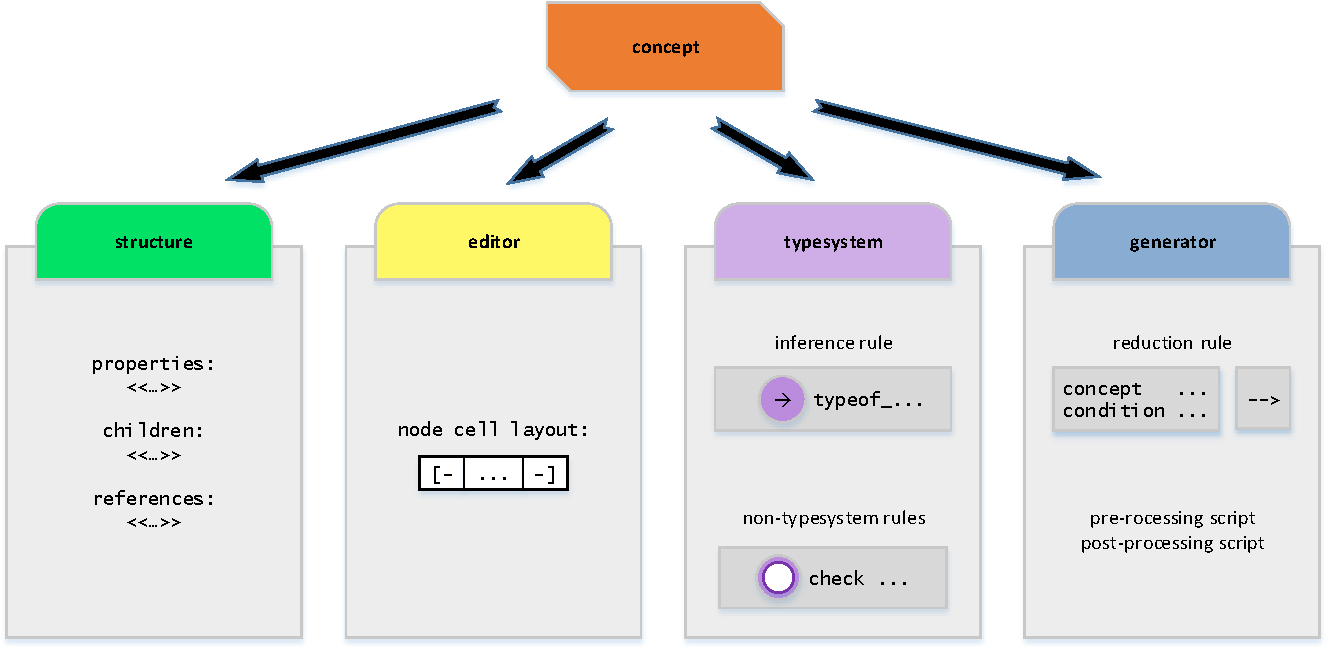
\includegraphics[scale=.78]{pics/MPS}
\caption{Concepts and language aspects in MPS}
\end{figure}

The complete definition of a concept comprises the definition of certain \textit{language aspects}: the structure of a concept is defined in a \textit{structure} aspect which contains the definition of the concept's abstract syntax in the abstract syntax tree (AST) of the program. The visual representation of the concept, its concrete syntax, is defined in the \textit{editor} aspect. The \textit{typesystem} aspect of a concept may contain a type inference rule for it and further \textit{non-typesystem rules}, which restrict the way it may be used. In a formal meta-language, the latter are usually part of the inference rules but are kept separately in MPS to diminish the complexity of inference rules and facilitate an easy extension of them. The \textit{generator} ``defines the denotational semantics for the concepts in the language'' \cite{GeneratorUserGuide}. Thus, this aspect describes the translation (in the following also called \textit{reduction} and \textit{transformation}) of concepts into concepts of the base language.
The implementation of C in mbeddr does not only provide extensions to the core of C but also offers a few differences to the basis of the C99 standard. They will be introduced as needed.

\subsubsection{C}
\label{cBasics}
The semantics of C differ from modern object-oriented languages like Java in various ways. In order to clarify some of the choices that were made for the design and implementation of ParallelMbeddr, in the following, the most relevant differences shall be outlined. Like Java, C leverages pass-by-value semantics for function parameters. In contrast to Java though, which copies the references themselves, C copies the referenced values into the memory that is allocated to the parameters of function calls. Thus, a change to a field of a structure (struct) instance that was copied in such a way does not affect the original struct instance.\footnote{The only way to avoid this behavior is to copy the memory addresses of values as pointers into functions.} On the other hand, arrays are treated like pointers, i.e. memory addresses as values, which becomes evident when they are passed to functions. Hence, a change of an entry of an array argument actually changes the array that is referred to by a variable on the caller site. For an array to be copied entirely into a function (not just by its address), it can be declared as a struct field, which, due to the copy semantics for structs, ensures that like any other field of the struct instance the array's value is copied into the newly created struct instance. The copy semantics are not restricted to function arguments but also extend to function return values and variable assignments. The `pass-by-pointer-value' semantics for arrays in C implies that arrays cannot be returned from functions as is done in Java. Instead, corresponding pointers are returned. This means that it is not safe to return an array, respectively a pointer thereof, from a function if the array resides in the area of the stack that was allocated for this function.\footnote{Otherwise the pointed-to memory of the returned array pointer would become deallocated after the return of the called function. This again would cause the return of a dangling pointer into the receiver of the returned value, i.e. a pointer that does not point to a valid memory address.} 
A peculiarity of C is that global variables may only be initialized with constant expressions, which makes it impossible to initialize a global variable with an arbitrary function call of a proper type \cite[p.~48]{CForBASICProgrammers}. In C, the type of a pointer to a value of type \CODE{t} is written \CODE{t*}.
